% *******************************************************************************
% * Copyright (c) 2007-2008 by Elexis
% * All rights reserved. This document and the accompanying materials
% * are made available under the terms of the Eclipse Public License v1.0
% * which accompanies this distribution, and is available at
% * http://www.eclipse.org/legal/epl-v10.html
% *
% * Contributors:
% *    G. Weirich - initial implementation
% *
% *  $Id: konsviews.tex 3329 2007-11-07 17:44:06Z rgw_ch $
% *******************************************************************************

% !Mode:: "TeX:UTF-8" (encoding info for WinEdt)
\section{Résultats dans Elexis}
\label{befunde}
\index{Résultats}\index{série de résultats Quick/TP}
Intégration des séries de résultats datés et classés selon le texte (par ex. poids, glycémie, Quick/TP, résultats radiologiques etc.) .
\subsection{Configuration}

\begin{figure}[htbp]
   \begin{minipage}{0.35\textwidth}
       \centering
       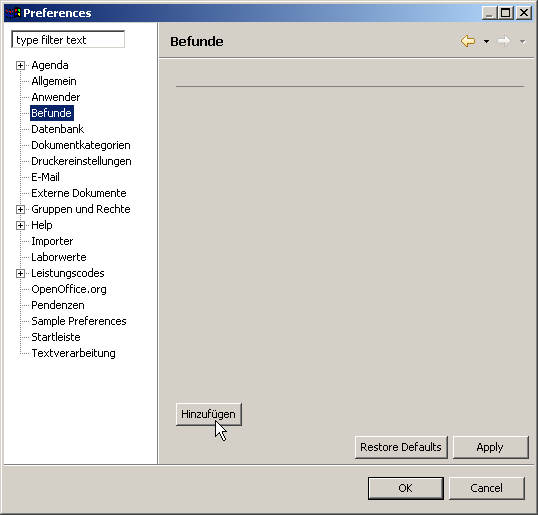
\includegraphics[width=0.9\textwidth]{images/befunde1}
       \caption{Befund}
       \label{fig:befundesettings}
     \end{minipage}\hfill
     \begin{minipage}{0.65\textwidth}
     Si ce Plugin est installé, vous trouvez dans le menu 'Fichier-Options' une rubrique  \textit{résultats}. Cette rubrique est probablement encore vide  (Fig. \ref{fig:befundesettings}).\\

     Pour ajouter un nouveau paramètre de résultats cliquez sur \textit{ajouter}. Vous serez ensuite demandé d'introduire le nom du paramètre. Nous avons choisi 'radiographie'. Il apparaîtra un onglet avec le nom du paramètre. Vous devez encore créer des champs pour l'introduction des données.

    \end{minipage}
\end{figure}
\begin{figure}[htbp]
   \begin{minipage}{0.35\textwidth}
       \centering
        % befunde2.png: 538x515 pixel, 96dpi, 14.23x13.62 cm, bb=0 0 403 386
       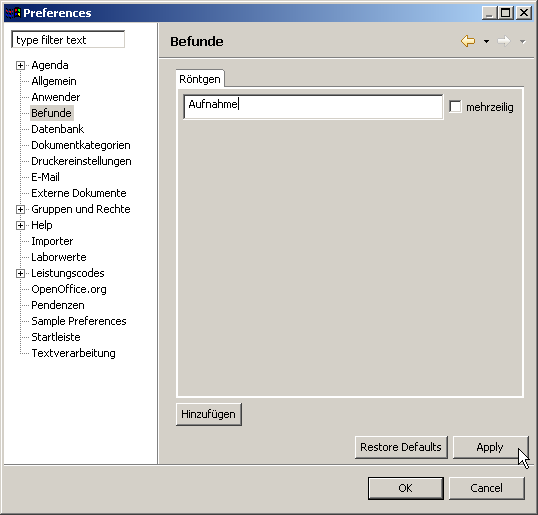
\includegraphics[width=0.9\textwidth]{images/befunde2}
       \caption{Parameter 2}
       \label{fig:befundesettings}
     \end{minipage}\hfill
     \begin{minipage}{0.65\textwidth}
        Cliquez après chaque ligne sur   \textit{Apply}  réspectivement  \textit{appliquer}:
        Si un champ doit contenir plusieurs lignes cliquez sur le 'checkbox' correspondante. Fig. \ref{fig:befunde4}vous montre une variante avec plus que deux lignes:

    \end{minipage}
\end{figure}
\begin{figure}[htbp]
   \begin{minipage}{0.35\textwidth}
       \centering
    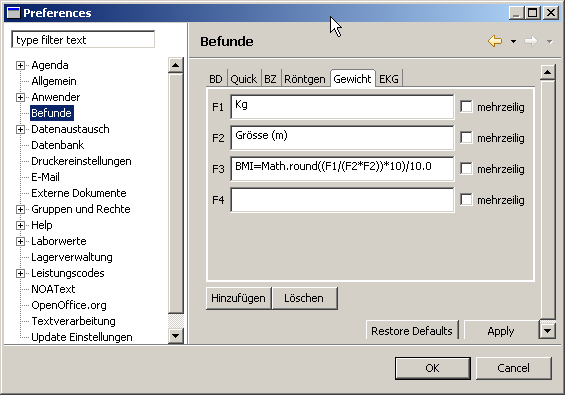
\includegraphics[width=0.9\textwidth]{images/befunde7.png}
    % befunde7.png: 580x520 pixel, 96dpi, 15.34x13.76 cm, bb=0 0 435 390
    \caption{Mehrspaltig}\label{fig:befunde4}
       \label{fig:befunde4}
     \end{minipage}\hfill
     \begin{minipage}{0.65\textwidth}
Certaines valeurs peuvent aussi être calculées au lieu d'être introduites directement. Vous pouvez introduire pour cela simplement une expression en forme de :  \textit{Résultat = Formule }, où par Fx vous pouvez vous référer à d'autres lignes de la même page. L'exemple à gauche montre comment calculer le BMI (indice de masse corporelle) avec les données introduites pour le poids et la taille. Le résultat est normalement affiché avec une exactitude à 9 chiffres, raison pour laquelle on l'arrondit à une décimale.
    \end{minipage}
\end{figure}

\clearpage

\subsection{Application}
Ouvrez le View des résultats .
\begin{flushleft}
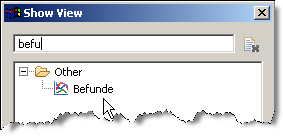
\includegraphics[width=3in]{images/befunde4.png}
% befunde4.png: 276x394 pixel, 96dpi, 7.30x10.42 cm, bb=0 0 207 295
\end{flushleft}

Vous y voyez les paramètres configurés pour les résultats:
\begin{flushleft}
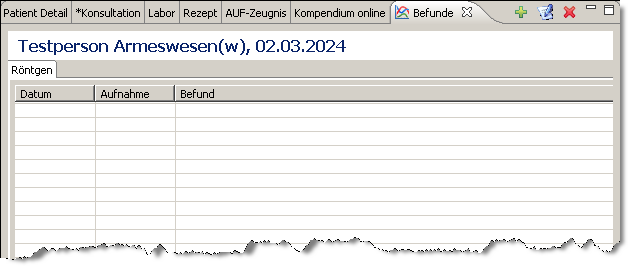
\includegraphics[width=4in]{images/befunde5.png}
% befunde5.png: 621x636 pixel, 96dpi, 16.43x16.83 cm, bb=0 0 466 477
\end{flushleft}
Pour y introduire des nouveaux résultats veuillez cliquer sur le plus vert à droite en haut. 
\begin{flushleft}
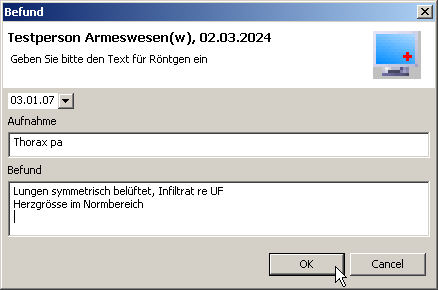
\includegraphics[width=3in]{images/befunde6.png}
% befunde6.png: 438x290 pixel, 96dpi, 11.59x7.67 cm, bb=0 0 328 217
\end{flushleft}
Vous pouvez voir maintenant les champs que vous avez introduits lors de la configuration pour y introduire vos résultats. Par un clique sur OK les données introduites seront intégrées. Avec un double-clique sur la ligne vous pouvez ouvrir les champs pour appliquer des corrections.

Si une valeur doit être calculée vous devez cliquer sur le titre en bleu pour que le calcul se fasse :\
\begin{center}
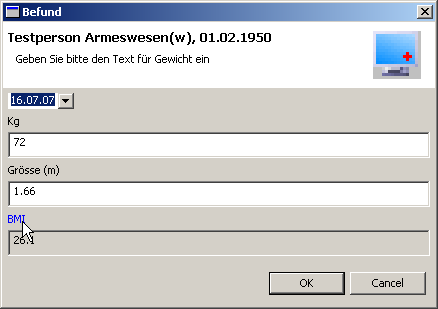
\includegraphics{images/befunde8}
\end{center}

\subsection{Variables dans un texte}
\index{variables} \index{variables dans un texte}
Les résultats peuvent aussi être introduits en forme de variables dans un document de texte. Pour cela vous pouvez appliquer la syntaxe comme c'est décrit sous (\ref{datenfelder_extern}, page \pageref{datenfelder_extern}). Le nom clé du plugin des résultats est : \textsc{Befunde-Data}.

Pour introduire dans un document par exemple un tableau avec l'historique de l'évolution du poids du patient actuel, vous introduisez les variables suivantes dans le texte :
\begin{verbatim}
    [Befunde-Data:Patient:all:Gewicht]  (pour introduire un tableau avec tout les mesures du poids)
    [Befunde-Data:Patient:last:Gewicht] (pour introduire seulement la dernière valeur du poids)
\end{verbatim}
